%4章提案
\begin{comment}
 そこで、新規に機器監視サービスを開発することにしました。
 今までの実践の中から要件を洗い出し、次のような物が必要となっていることがわかりました。
 この要件から、機能を洗い出してみました
\end{comment}
そこで、新規にIoT機器の監視に汎用的に使用できるシステムを開発し、サービスとして提供することで、問題の解決が図れるのではないかと考えた。
実験と聞き取りから得られた要件となるを以下にまとめる。
\begin{itemize}
\item 機器が接続するネットワークの設定を変更することは出来ない
\item 店舗ネットワーク及びSORACOMAirのネットワークでは、プライベートアドレスが利用されているため、インターネットから観測機器にアクセスすることが出来ない
\item 提供しているサービスに監視機能を組み込む事が難しい
\item 新規に監視サーバを立ち上げる事が負担となる
\item 単純に機器が起動し、動作している事が確認できれば良い
\item 欲を言うと、CPUの温度等も確認できれば良い
\item 各機器に対するVPNや監視の為の設定も簡略化できたら尚良い
\end{itemize}

\section{IoT機器監視サービスの機能}
前項の要件から、必要となる機能を次にまとめた。
\begin{itemize}
\item 
\end{itemize}
また、制約を次にまとめる。
\begin{itemize}
\item 
\end{itemize}


\begin{comment}
\section{IoT機器の監視}%3.1
%(ここにおける監視とはどういったものなのか,どのような状態を監視しなければならないのか,また,監視において何をしなければならないのか,何が起きたらどう対処しなければならないのか,何故そうしなければならないのか)

IoT機器の監視とは,動作の状態・通信の状態を確認することである.
IoT機器の動作の状態・通信の状態を確認し,記録することは,IoTサービスを維持する上で重要である.
動作状態とは,少なくとも電源が入っているのかどうかで,通信状態とは,インターネットに接続され,サーバーと通信ができているのかどうかである.
\medskip

このように,個々のIoT機器の動作状態,通信状態を確認し,記録することが,IoT機器の監視である.

\section{IoT機器監視の重要性と問題点}
IoT機器の監視は,IoTサービスを停止させないために重要である.
IoT機器が正常に動作していない事が分かった場合,正確に分析できないため,サービスを提供することができなくなる.
そのために,常にIoT機器を監視し,異常が有れば,復旧作業を行う必要がある.
また,IoT機器が正常に動作していない場合,分析を正確なものとするため,分析時に該当のIoT機器を除外するか,全てのIoT機器が動作している時間帯を選び分析を行う必要がある.
そのため,IoT機器を監視し,IoT機器が正常に動作していない時間を記録しておく必要がある.
\medskip

このようにIoT機器の監視は,IoTサービスを維持する上で重要である.
しかし,従来より用いられてきた手法は,様々なネットワークに接続されるIoT機器の特性上用いることは難しい.
また,機器が非常に安価になっていく事を考えると,機器の設定に手間を掛けたくない.

\section{IoT機器からの通知に基づく機器監視サービスの提案}
そこで私は,IoT機器の監視に特化したIoT機器監視サービスのを提案する.
IoT機器から機器監視サーバに通知を送ることで,IoT機器が接続されるネットワークによらない機器監視が行えると考えた.
IoT機器の監視に特化させることで,機器の監視に手間をかけずにすむようになると考える.
図\ref{fig:proposal_system}は提案サービスの図である.

\begin{figure}[htbp]
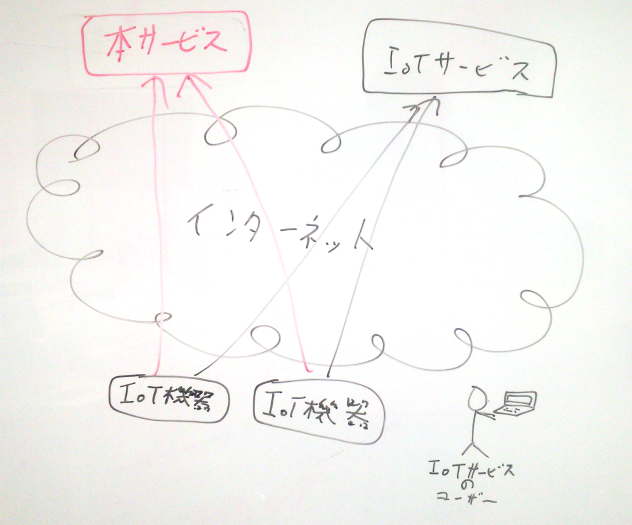
\includegraphics[width=14cm]{images/proposal_system.png}
\caption{IoTサービスの構成図}
\label{fig:proposal_system}
\end{figure}

構成として、次のような特徴を持つ。
\begin{itemize}
	\item 機器から通知を送る\\
		そのため、NAPTの影響をうけない。
	\item IoTサービスと独立して監視を行う\\
		そのため、IoTサービスを変更する必要が無い。
\end{itemize}

\section{IoT機器の監視における要件}%3.2
%(どのような制約条件が存在するのか,何故そのような制約が発生するのか)
IoT機器の監視には,上記機能が必要である他に,IoT機器が設置されるネットワークにかかわらず監視ができることが求められる.
何故ならば,IoT機器が設置されるネットワーク環境は多様であるからである.
\medskip

IoT機器が設置されるネットワーク環境として,次のような環境が挙げられる.
\begin{itemize}
	\item IoT機器に対しプライベートアドレスが与えられる環境
	\item IoT機器とサーバーの通信が制限される環境
\end{itemize}

多くの場合,IPアドレスの節約の観点から,IoT機器に対し,プライベートアドレスのみ与えられる.
この場合,インターネット側からは,IPアドレスを指定することが出来ないため,通信は常にIoT機器から始まる必要がある.
また,IoT機器とサーバーとの通信がセキュリティの観点から制限される場合もある.
HTTP等一般的に広く使用される通信を除いてブロックされる事がある.
\medskip

このようにIoT機器の監視には,IoT機器から通信が始まることや,HTTP等頻繁に利用される通信を利用しなければならないといった制約がある.




%(機器監視に求められる要件を整理し,述べる)
これらを踏まえて,IoT機器の監視には次のような機能要件が求められる.
\begin{itemize}
	\item IoT機器の動作状態,通信状態を検知する機能
	\item IoT機器の動作状態,通信状態を記録する機能
	\item IoT機器の動作状態を一覧して表示する機能
	\item IoT機器の過去の状態を確認する機能
\end{itemize}
また,非機能要件として,次のような制約がある.
\begin{itemize}
	\item プライベートアドレスが与えられたとしても動作する事
	\item インターネットの通信として一般に広く利用されているHTTP等の通信を用いる事
	\item IoTサービスへの変更が無い事
	\item IoT機器への設定が簡単である事
\end{itemize}


\section{IoT機器の監視に必要な機能}%3.2
%(どのような機能が必要となるのか,IoT機器の状態を一覧して表示することとはどういったことなのか,IoT機器の過去の状態を監視することができるとはどういったことなのか,何故そのような機能が必要なのか)
IoT機器の監視とは,個々のIoT機器の動作状態,通信状態を確認することである.
そのため,次のような機能が必要となる.
\begin{itemize}
	\item IoT機器の動作状態,通信状態を検知する機能
	\item IoT機器の動作状態,通信状態を記録する機能
	\item IoT機器の動作状態を一覧して表示する機能
	\item IoT機器の過去の状態を確認する機能
\end{itemize}

IoT機器の動作状態,通信状態を検知する機能とは,IoT機器の現在の状態を検知する機能である.

IoT機器の動作状態,通信状態を記録する機能とは,IoT機器の状態を時刻と共に記録する機能である.

IoT機器の動作状態を一覧して表示する機能とは,現在のIoT機器の動作状態を見ることができる機能である.
あるIoT機器が動作しなくなった時に,動作していないことを明確に示す必要がある.
\medskip

IoT機器の過去の状態を確認する機能とは,過去のIoT機器の動作状態と通信状態を確認することができる機能である.
過去の動作状態や通信状態を整理し,いつ動作していて,いつ動作していなかったのか,各IoT機器ごとに示す必要がある.
\medskip

このように,IoT機器の監視には,IoT機器の動作状態を一覧して表示する機能,IoT機器の過去の状態を確認する機能を持つ必要がある.

\end{comment}










